% 2003 年江苏卷第 1 题：点 (a, b) 区域选项图
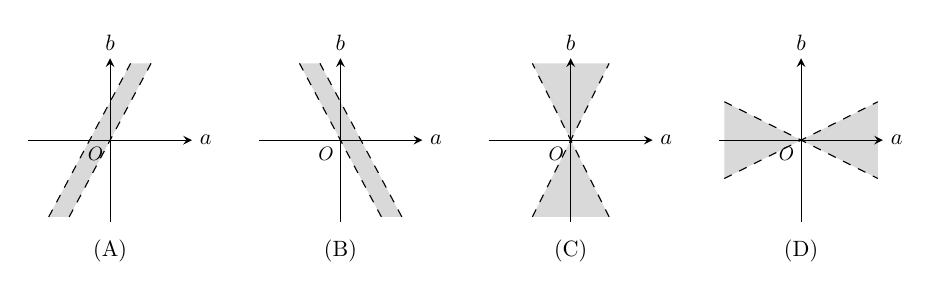
\begin{tikzpicture}[>=stealth,scale=0.65]
  % A
  \begin{scope}[shift={(0,0)}]
    \fill[black!15] (-1.2,-1.5) -- (-0.8,-1.5) -- (0.8,1.5) -- (0.4,1.5) -- cycle;
    \draw[->] (-1.6,0) -- (1.6,0) node[right,scale=0.8] {$a$};
    \draw[->] (0,-1.6) -- (0,1.6) node[above,scale=0.8] {$b$};
    \node[below left,scale=0.7] at (0,0) {$O$};
    \draw[dashed] (-1.2,-1.5) -- (0.4,1.5);
    \draw[dashed] (-0.8,-1.5) -- (0.8,1.5);
    \node[below,scale=0.8] at (0,-1.8) {(A)};
  \end{scope}

  % B
  \begin{scope}[shift={(4.5,0)}]
    \fill[black!15] (1.2,-1.5) -- (0.8,-1.5) -- (-0.8,1.5) -- (-0.4,1.5) -- cycle;
    \draw[->] (-1.6,0) -- (1.6,0) node[right,scale=0.8] {$a$};
    \draw[->] (0,-1.6) -- (0,1.6) node[above,scale=0.8] {$b$};
    \node[below left,scale=0.7] at (0,0) {$O$};
    \draw[dashed] (1.2,-1.5) -- (-0.4,1.5);
    \draw[dashed] (0.8,-1.5) -- (-0.8,1.5);
    \node[below,scale=0.8] at (0,-1.8) {(B)};
  \end{scope}

  % C
  \begin{scope}[shift={(9,0)}]
    \fill[black!15] (0,0) -- (0.75,1.5) -- (-0.75,1.5) -- cycle;
    \fill[black!15] (0,0) -- (0.75,-1.5) -- (-0.75,-1.5) -- cycle;
    \draw[->] (-1.6,0) -- (1.6,0) node[right,scale=0.8] {$a$};
    \draw[->] (0,-1.6) -- (0,1.6) node[above,scale=0.8] {$b$};
    \node[below left,scale=0.7] at (0,0) {$O$};
    \draw[dashed] (-0.75,-1.5) -- (0.75,1.5);
    \draw[dashed] (0.75,-1.5) -- (-0.75,1.5);
    \node[below,scale=0.8] at (0,-1.8) {(C)};
  \end{scope}

  % D
  \begin{scope}[shift={(13.5,0)}]
    \fill[black!15] (0,0) -- (1.5,0.75) -- (1.5,-0.75) -- cycle;
    \fill[black!15] (0,0) -- (-1.5,0.75) -- (-1.5,-0.75) -- cycle;
    \draw[->] (-1.6,0) -- (1.6,0) node[right,scale=0.8] {$a$};
    \draw[->] (0,-1.6) -- (0,1.6) node[above,scale=0.8] {$b$};
    \node[below left,scale=0.7] at (0,0) {$O$};
    \draw[dashed] (-1.5,-0.75) -- (1.5,0.75);
    \draw[dashed] (-1.5,0.75) -- (1.5,-0.75);
    \node[below,scale=0.8] at (0,-1.8) {(D)};
  \end{scope}
\end{tikzpicture}
